\documentclass[paper = A5, headinclude, parskip = full, oneside, font = 11 pt]{report}

%==========================================================================================================================

%Cover Page
 \title{\textit{\textbf{\emph{P}}rogramming \textbf{\emph{W}}ith \textbf{\emph{J}}ava}}
 \author
 {
 	\textbf{Sofiullah Iqbal Kiron}
 	\\
 	CSE, BSMRSTU\{SHIICT\}
 	\\
 	\\
 	E-mail 1: \href{mailto:sofiul.k.1023@gmail.com}{sofiul.k.1023@gmail.com}
 	\and
 	E-mail 2: \href{mailto:kiron.1023.s@gmail.com}{kiron.1023.s@gmail.com}
 }
 \date{27 December, 2019}

%>>>>>>>>>>>>>>>>>>>>>>>>>>>>>>>>>>>>>>>>>>>>>>>>>>>>>>>>>>>>>>>>>>>>>>>>>>>>>>>>>>>>>>>>>>>>>>>>>>>>>>>>>>>>>>>>>>>>>>>>>>

%Packages
 %Color and graphical packages
	\usepackage{graphicx, xcolor, subfigure}
 %Graph-art packages
	\usepackage{tkz-graph, pgfplots}
 %Coloured boxing packages
 	\usepackage[english]{babel}
 	\usepackage[pangram]{blindtext}
 	\usepackage{tcolorbox}
 %Coding package
	\usepackage{listings}
	\lstset
    {
	 tabsize = 4,
	 showstringspaces = false,
	 numbers = left,
	 commentstyle = \color{green}
	 keywordstyle = \color{blue}
	 stringstyle = \color{red}
	 rulecolor = \color{black}
	 basicstyle = \small \ttfamily
	 breaklines = true,
	 numberstyle = \tiny
	}
 %Other packages
 	\usepackage{hyperref, courier}

%**************************************************************************************************************************

\begin{document}

\pagecolor{green}

\maketitle
\frenchspacing
\pagenumbering{roman}
\pagestyle{plain}

\pagecolor{white}

\begin{abstract}
\color{blue}
\emph{O}bject never automatically oriented. So, orient the object.\\
Go with Java, start with "Hello World!"
\color{black}
\end{abstract}

\newpage

\pagecolor{black!89}

\begin{center}
 \color{violet}
  WORA - WRITE ONCE, RUN ANYWHERE
 \color{black}
 
 \begin{huge}
 \color{white}
  This is a simple \textbf{\LaTeX{}} file.
 \end{huge}
\end{center}

\begin{center}
\color{brown}
{\LARGE Instructed by: \textbf{Honorable Nasif Ahamed}\\Lecturer, dept. of CSE.}
\end{center}

\newpage

\pagecolor{white}

\color{black}
\section*{Introduction}
\textbf{P}rogramming is not a specific said that it is abounded in the computer science or software development in mobile, computers, macro gadgets or others electronic device. Programming is with all around the world. The solar system of our galaxy (named, \textit{Milki Way galaxy}) is also a program for define the path-walk of all planets. Our sun solar system is also a great program. Program is in everywhere as possible places we looking after. Our daily life is a program for featuring all purposes and goal.
\\

At first, pepoles assume that "\textbf{\textit{Ada Lavlas}}" is the first program writer in the world. For his respect, there stayed a programming language namely "\textbf{Ada}".
\\
Ada was doughter of a peris poet.
\\
\\
Here, in this report document, I'm gonna briefly telling about the most powerful programming language, which has been dominated above on other programming languages.
\\
So, let's get started...
\begin{flushright}
 Sofiullah Iqbal Kiron.
 \\
 dept. of CSE,\\BSMRSTU(SHIICT)
 \\
 \date{\today}
\end{flushright}

\newpage

\tableofcontents

\newpage

%Chapter one
\chapter{Primary discussion}
Programming languages are evaluated from many of days.

%First Section
\color{green}
\section{Top programming languages}
\color{black}
\textbf{H}ere I'm gonna briefly telling about some top programming languages...\\

At first, Let's see a simple table for this index:-

\begin{center}

%Table 1, start.
 \begin{tabular}{||c|c|c|c|c||}

 \hline
 \hline
 1. Python & 2. Java & 3. JavaScript & 4. C/C++ & 5.GoLang\\
 \hline
 6. R & 7. Kotlin & 8. C\# (C Sharp) & 9. Swift & 10. PHP\\
 \hline
 \hline
 
 \end{tabular}
%Table 1, over.

\end{center}

%1.1.1
\subsection{Python}
\emph{\textit{\large{P}}}ython is the world first popular programming language by users of coders community. Python as developed by "Guido Van Rossum" in the year of 1991. Python is interpreted, high-level, general-purpose programming language. Python's design philosophy emphasizes code readability with its notable use of significant white-space. Python is dynamically typed and garbage-collected. It supports multiple programming paradigms, including procedural, object-oriented, and functional programming. Python is often described as a "batteries included" language due to its comprehensive standard library. I'm gonna briefly describe java with a simple graphical chart picture. 
\begin{center}
 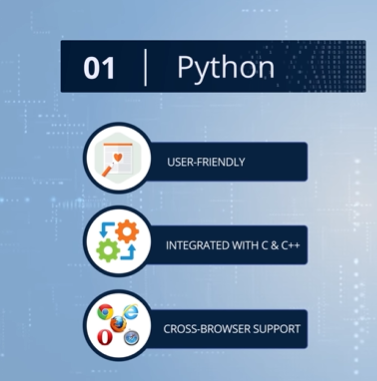
\includegraphics[width = 140 pt]{Python.png}
\end{center}

%1.1.2
\subsection{Java}
\emph{\textit{\large{J}}}ava is also a general purpose, object oriented programming language that was developed by "Sun Microsystem" and designed by "James Gosling". Java is a general-purpose programming language that is class-based and designed to have as few implementation dependencies as possible. It is intended to let application developers write once, run anywhere (\textbf{WORA}), meaning that compiled Java code can run on all platforms that support Java without the need for recompilation.[16] Java applications are typically compiled to byte-code that can run on any Java virtual machine (JVM) regardless of the underlying computer architecture. The syntax of Java is similar to C and C++, but it has fewer low-level facilities than either of them. As of 2019, Java was one of the most popular programming languages in use according to GitHub, particularly for client-server web applications, with a reported 9 million developers.
\begin{center}
 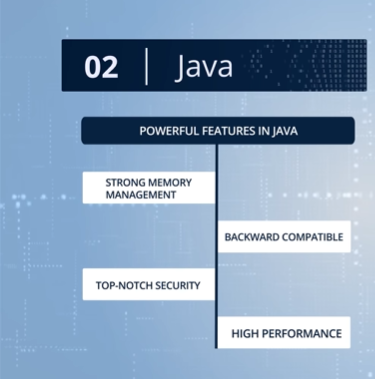
\includegraphics[width = 140 pt]{Java.png}
\end{center}

%1.1.3
\subsection{JavaScript}
\emph{\textit{\large{J}}}avaScript also third and more popular and high-designed programming language. Its often abbreviated as \textbf{JS}, is a high-level, just-in-time compiled, object-oriented programming language that conforms to the ECMAScript specification. JavaScript has curly-bracket syntax, dynamic typing, prototype-based object-orientation, and first-class functions.

Alongside \textit{HTML} and \textit{CSS}, JavaScript is one of the core technologies of the World Wide Web. JavaScript enables interactive web pages and is an essential part of web applications. The vast majority of websites use it, and major web browsers have a dedicated JavaScript engine to execute it.
\begin{center}
 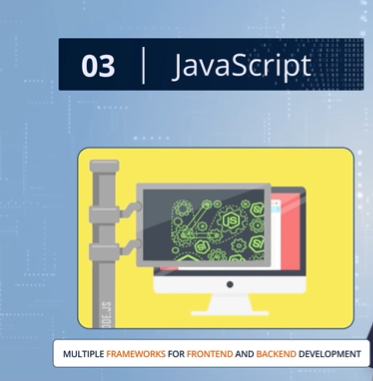
\includegraphics[width = 140 pt]{JavaScript.png}
\end{center}

%1.1.4
\subsubsection{C/C++}
\subsubsection{C}
Most of languages are mainly based on basic structure of the language C and C++. C is the greatest 'Structured Programming Language' of all over the priority. is a general-purpose, procedural computer programming language supporting structured programming, lexical variable scope, and recursion, while a static type system prevents unintended operations. By design, C provides constructs that map efficiently to typical machine instructions and has found lasting use in applications previously coded in assembly language. Such applications include operating systems and various application software for computers, from supercomputers to embedded systems. C was originally developed at Bell Labs by "\textbf{Dennis Ritchie}" between \textit{1972} and \textit{1973} to make utilities running on Unix. Later, it was applied to re-implementing the kernel of the Unix operating system.

\subsubsection{C++}
C++ is the greatest "Object Oriented Programming Language" that was developed by "Bjarne Stroustup". He said that, 'C++' basically is a extension of C. The '++' sign is taken from the increment operator of C programming language. The language - C++ firstly named 'C with classes'. After evolution the times, stroustup assume that it's not a proper name. Than, ending of ANSI committee, he changed the name of this language as C++. Basically the concept of class is taken from of the 'Structure' concept of language C. Now, C++ is most popular language that are using for many computational function.
\begin{center}
 
\includegraphics[width = 140 pt]{C++ Logo.png}
\end{center}

%Chapter Two
\chapter{Starting With Java}

%First Section(2.1)
\color{green}
\section{Java, as a programming Language}

\color{black}
\textbf{A}s a programming language, we can simply assume that, Java is a powerful programming language. Great for all general purpose for develop of software.
Let's see compilation system of Java compiler:-
\\
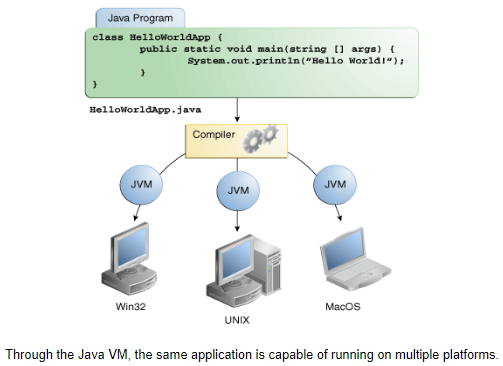
\includegraphics[width = 230 pt]{Compilation system.png}

\newpage

%Second Section(2.2)
\color{green}
\section{Features of Java}

\color{black}
\textbf{T}he Java programming language is a high-level language that can be characterized by all of the following topic-words:-

\begin{itemize}
 \item Simple
 \item Object Oriented
 \item Distributed
 \item Multithreaded
 \item Dynamic
 \item Architecture
  \begin{itemize}
   \item Neutral
   \item Biased
  \end{itemize}
 \item Portable
 \item High Performance
 \item Robust
 \item Secure
\end{itemize}

not only those, java has more than features from those, which made java a more developed cross platfrom super level high performed and multipurpose language also, and so on...

%Fourth Section
\color{green}
\section{Java Development Software}

\color{black}
\textbf{T}here are many kind of Java Development Kits were developed, means compiler for java. Such as:

\begin{enumerate}
 \item NetBeans
 \item Eclipse
 \item JDK
 \item JRE
 \item IntelliJ IDEA
\end{enumerate}

and many other development or compiler kits are available for writing and compiling for java codes.
\\
\\
Let's describe all of this itemized kits of java at several subsections...

\color{red}
\subsection{NetBeans}
\color{black}
\textit{NetBeans}: NetBeans is an integrated development environment for Java. NetBeans allows applications to be developed from a set of modular software components called modules. NetBeans runs on Windows, macOS, Linux and Solaris. Author of this software - " Roman Staněk ".

\begin{center}
 
\includegraphics[width = 140 pt]{NetBeans.png}
\end{center}

\color{red}
\subsection{Eclipse}
\color{black}
\textit{Eclipse}: Eclipse is an integrated development environment used in computer programming. It contains a base workspace and an extensible plug-in system for customizing the environment. It was owned by - "Eclipse Foundation".

\begin{center}
 
\includegraphics[width = 140 pt]{Eclipse.png}
\end{center}

\color{red}
\subsection{JDK}
\color{black}
\textit{JDK}: The Java Development Kit is an implementation of either one of the Java Platform, Standard Edition, Java Platform, Enterprise Edition, or Java Platform, Micro Edition platforms released by Oracle Corporation in the form of a binary product aimed at Java developers on Solaris, Linux, macOS or Windows. It was developed by - " Oracle Corporation".

\begin{center}
 
\includegraphics[width = 140 pt]{JDK.png}
\end{center}

\color{red}
\subsection{JRE}
\color{black}
\textit{JRE}: JRE a basic platform of running the Java code. If we don't want to run code of Java but not develop to a software, than we can easily use this software.

\begin{center}
 
\includegraphics[width = 140 pt]{JRE.png}
\end{center}

\color{red}
\subsection{IntelliJ IDEA}
\color{black}
\textit{IntelliJ IDEA}: IntelliJ IDEA is an integrated development environment written in Java for developing computer software. It is developed by JetBrains, and is available as an Apache 2 Licensed community edition, and in a proprietary commercial edition. Both can be used for commercial development.

\begin{center}
 
\includegraphics[width = 140 pt]{IntelliJ IDEA.png}
\end{center}

%Fourth section(2.4)
\color{green}
\section{A Simple Java Program}
\color{black}
Here, illustrating a simple java program...

\color{purple}
\begin{lstlisting}[language = Java, frame = trBL, firstnumber = last, escapeinside = {(*@}{@*)}]
public class Factorial
{
    public static void main(String[] args)
    {   final int NUM_FACTS = 100;
        for(int i = 0; i < NUM_FACTS; i++)
            System.out.println( i + "! is " + factorial(i));
    }

    public static int factorial(int n)
    {   int result = 1;
        for(int i = 2; i <= n; i++) (*@\label{for}@*)
            result = result * i;
        return (result);
    }
}
\end{lstlisting}

%Fifth section
\color{green}
\section{James Gosling}
\color{black}
\textbf{W}e passed many time by writing about Java codes but still, means even we don't talk about the designer of "Java" at least a single line, he is "James Gosling".
James Gosling is a Canadian computer scientist, best known as the founder and lead designer behind the Java programming language.

%Subsection (2.5.1)
\color{red}
\subsection{Education Qualification and Carrier Lines}
\color{black}
\textbf{J}ames Gosling received a Bachelor of Science from the University of Calgary and his M.A. and Ph.D. from Carnegie Mellon University, all in computer science. He wrote a version of Emacs called Gosling Emacs (Gosmacs) while working toward his doctorate. He built a multi-processor version of Unix for a 16-way computer system while at Carnegie Mellon University, before joining Sun Microsystems. He also developed several compilers and mail systems there.

Gosling was with Sun Microsystems between 1984 and 2010 (26 years). He is known as the father of the Java programming language. He got the idea for the Java VM while writing a program to port software from a PERQ by translating Perq Q-Code to VAX assembler and emulating the hardware. He left Sun Microsystems on April 2, 2010 after it was acquired by the Oracle Corporation, citing reductions in pay, status, and decision-making ability, along with change of role and ethical challenges. He has since taken a very critical stance towards Oracle in interviews, noting that "during the integration meetings between Sun and Oracle, where we were being grilled about the patent situation between Sun and Google, we could see the Oracle lawyer's eyes sparkle." He clarified his position during the Oracle v. Google trial over Android: "While I have differences with Oracle, in this case, they are on the right. Google totally slimed Sun. We were all really disturbed, even Jonathan Schwartz; he just decided to put on a happy face and tried to turn lemons into lemonade, which annoyed a lot of folks on Sun." However, he approved of the court's ruling that APIs should not be copyrightable.

In March 2011, Gosling left Oracle to work at Google. Six months later, he followed his colleague Bill Vass and joined a startup called Liquid Robotics. In late 2016, Liquid Robotics was acquired by Boeing. Following the acquisition, Gosling left Liquid Robotics to work at Amazon Web Services as Distinguished Engineer in May 2017.

He is an advisor at the Scala company Lightbend, Independent Director at Jelastic, and Strategic Advisor for Eucalyptus, and is a board member of DIRTT Environmental Solutions.

He is known for his love of proving "the unknown" and has noted that his favorite irrational number is $\sqrt{2}$. He has a framed picture of the first 1,000 digits of $\sqrt{2}$ in his office.

%Subsection (2.5.2)
\color{red}
\subsection{Contribution of James gosling}
\color{black}
\textbf{G}osling initially became known as the author of Gosling Emacs. He also invented an early Unix windowing system called NeWS, which became a lesser-used alternative to the still used X Window, because Sun did not give it an open source license.[citation needed] He is generally credited with having invented the Java programming language in 1994. He created the original design of Java and implemented the language's original compiler and virtual machine. Gosling traces the origins of the approach to his early graduate student days, when he created a p-code virtual machine for the lab's DEC VAX computer, so that his professor could run programs written in UCSD Pascal. In the work leading to Java at Sun, he saw that architecture-neutral execution for widely distributed programs could be achieved by implementing a similar philosophy: always program for the same virtual machine.
For his achievement, the National Academy of Engineering in the United States elected him as a Foreign Associate member. Another contribution of Gosling's was co-writing the "bundle" program, known as "shar", a utility thoroughly detailed in Brian Kernighan and Rob Pike's book The Unix Programming Environment.

%Section (2.6)
\color{red}
\section{Some Pictures of James Gosling}
\color{black}
\textbf{H}ere are a album for illustration of "\textit{James Gosling}" 's picture...

\newpage

\begin{center}

 \begin{figure}

 \begin{tcolorbox}[colframe = yellow, colback = green!89]

   \subfigure[James Gosling]{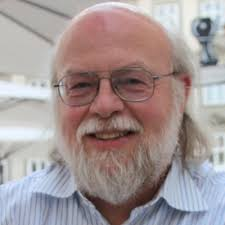
\includegraphics[width = 100 px]{James Gosling 1.jpg}}
   \subfigure[Designer of Java]{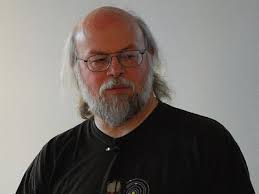
\includegraphics[width = 100 px]{James Gosling 2.jpg}}
   \subfigure[Computer Scientist]{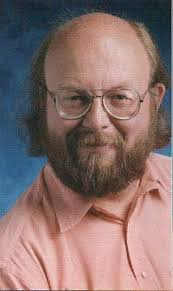
\includegraphics[width = 100 px]{James Gosling 3.jpg}}
   \subfigure[Language Developer]{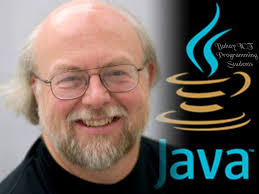
\includegraphics[width = 100 px]{James Gosling 4.jpg}}
 
 \end{tcolorbox}
 
 \end{figure}

\end{center}

%Chapter Three
\chapter{Closing Point}

\textbf{A}t the ending point or closing point of this \emph{\LaTeX{}} file, i just wanna say, there are upto \emph{Thousands} of programming languages and all are preferable above one up other. So, no one language are throwable. We need to learn most of them topper languages and must need to know how to solve the problems and implement those.
\\
Goodbye today, Best wishes for all.

\begin{tcolorbox}[colback = blue!35, colframe = black]
 \centering
 The End
\end{tcolorbox}

\end{document}